% 1977 年贵州卷第三题：直角三角形 ABC（∠ABC=90°），以直角边 AB 为直径作园，
% 园与斜边 AC 交于 D，过 D 的切线交 BC 于 E（切线向 D 上方延长），
% 虚线为辅助线 BD；角标注 ∠1（CDE）、∠2（DCE）、∠3（EDB）、∠4（DBE），
% B 处另画直角记号（按源卷第 3 页布局，几何关系自洽：ED=EB=3）
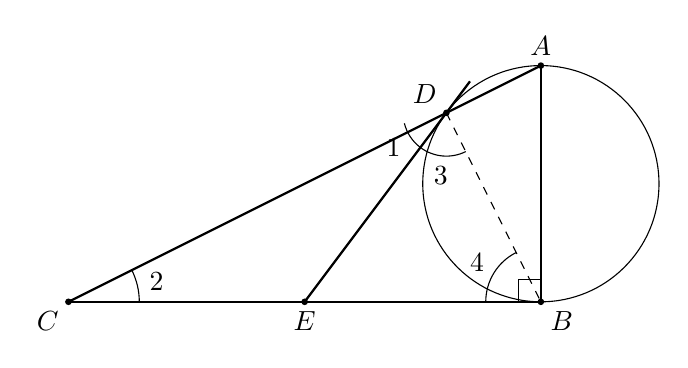
\begin{tikzpicture}[scale=1.0]
  \coordinate (B) at (0,0);
  \coordinate (A) at (0,3);
  \coordinate (C) at (-6,0);
  \coordinate (O) at (0,1.5);
  \coordinate (D) at (-1.2,2.4);
  \coordinate (E) at (-3,0);
  \coordinate (T) at (-0.9,2.8);
  \draw (O) circle (1.5);
  \draw[thick] (C)--(A);
  \draw[thick] (A)--(B);
  \draw[thick] (C)--(B);
  \draw[thick] (E)--(T);
  \draw[dashed] (D)--(B);
  \fill (A) circle (1.2pt) node[above] {$A$};
  \fill (B) circle (1.2pt) node[below right] {$B$};
  \fill (C) circle (1.2pt) node[below left] {$C$};
  \fill (D) circle (1.2pt) node[above left] {$D$};
  \fill (E) circle (1.2pt) node[below] {$E$};
  % ∠2（C 处，CB 与 CA 之间）
  \draw ([shift={(0:0.9)}]C) arc (0:26.57:0.9);
  \node at (-4.88,0.26) {$2$};
  % ∠1（D 处，DC 与 DE 之间）
  \draw ([shift={(194.04:0.55)}]D) arc (194.04:233.13:0.55);
  \node at (-1.87,1.96) {$1$};
  % ∠3（D 处，DE 与 DB 之间）
  \draw ([shift={(233.13:0.55)}]D) arc (233.13:296.57:0.55);
  \node at (-1.27,1.60) {$3$};
  % ∠4（B 处，BD 与 BC 之间）
  \draw ([shift={(116.57:0.7)}]B) arc (116.57:180:0.7);
  \node at (-0.81,0.50) {$4$};
  % B 处直角记号（∠ABC=90°）
  \draw (0,0.28)--(-0.28,0.28)--(-0.28,0);
\end{tikzpicture}
